
\section{Progettazione Concettuale}
Questa fase è di cruciale importanza poiché definisce il contenuto informativo del data mart. Tutta la prima parte di questa fase si occupa di capire qual è il modello che viene utilizzato, quindi individuare i vari costrutti che si potranno utilizzare. Non vi è uno standard ufficiale per la realizzazione della parte di progettazione concettuale del data mart. È possibile utilizzare il modello E-R per il data mart? No, perché è troppo espressivo e perché è nato per modellare realtà di business fatte in qualunque modo. Qui il modello deve essere multidimensionale e bisogna rispettare dei vincoli; quindi, ci devono essere gerarchie progettate in un certo modo. Molti progettisti disegnano direttamente gli schemi a stella (schemi logici relazionali). Questo tipo di approccio non è conveniente e funziona male perché racchiude solo la definizione di un insieme di relazioni e di vincoli di integrità (sono denormalizzate in pratica). 

Il formalismo che bisogna utilizzare si chiama \textbf{Dimensional Fact Model (DFM}). Ha una larga diffusione nei contesti italiani ed esteri, ma soprattutto nel mondo della ricerca. È un modello concettuale grafico pensato per:
\begin{itemize}
	\item 
	Supportare efficacemente il progetto concettuale
	\item 
	Permette di verificare che le interrogazioni (query OLAP) siano effettivamente esprimibili sul cubo che stiamo disegnando 
	\item 
	Supportare un dialogo tra progettista e utente finale
	\item 
	È fondamentale per la documentazione che deve essere espressiva e non ambigua
	\item 
	Creare una piattaforma stabile da cui partire per il progetto logico
\end{itemize}

Quando si utilizza il \textbf{DFM} creiamo degli schemi detti schemi di fatto. Trattandosi di schemi multidimensionali, ovviamente, disegneremo fatti, misure e gerarchie. Distingueremo la parte del DFM in costrutti di base e costrutti avanzati. I primi coprono un pò di più dell’espressività del modello multidimensionale. I secondi, invece, servono per modellare le sfumature che si incontrano nei progetti reali. 
\subsection{I costrutti di base}
\begin{itemize}
	\item
	\textbf{Fatto}: è un fenomeno di business che accade dinamicamente all’interno dell’azienda. È essenziale che un fatto abbia aspetti dinamici, ovvero evolva nel tempo
	\item 
	\textbf{Dimensione}: attributi numerici che quantificano il fatto da un certo punto di vista (il voto di laurea, qtà acquistata)
	\item 
	\textbf{Misura}: coordinate di accesso al cubo. 
\end{itemize}
\begin{figure}[H]
	\centering
	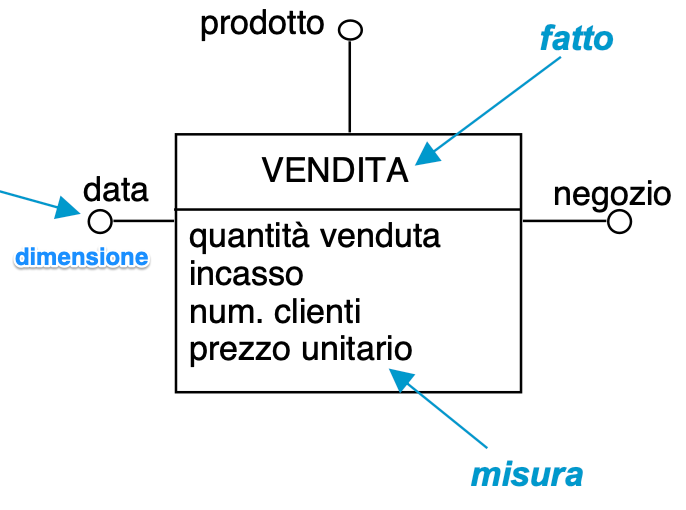
\includegraphics[width=0.7\linewidth]{img/example_fatto}
	\caption{Esempio di ...}
	\label{fig:exfatto}
\end{figure}
Quindi il tipo di relazione che ho tra prodotto, data e negozio è una classica associazione molti a molti. Dunque, un \textbf{fatto} esprime una associazione molti a molti tra le dimensioni.

Una \textbf{gerarchia} è una sequenza di attributi collegati tra di loro da associazioni molti ad uno, ossia da dipendenze funzionali. Le gerarchie non sono necessariamente dei percorsi, ma possono avere forme più complesse. In particolare possono essere degli alberi, i cui nodi si chiamano attributi dimensionali, i quali descrivono le dimensioni in modo via via più aggregato. L’\textbf{albero} non orientato è un grafo aciclico. In quest' albero la radice è la dimensione, mentre gli archi rappresentano dipendenze funzionali. 

Un \textbf{evento primario} è una particolare occorrenza di un fatto, individuata da una ennupla costituita da un valore per ciascuna dimensione. A ciascun evento primario è associato un valore per ciascuna misura. Per modellare il concetto dell’aggregazione sul DFM si ragiona in termini di group-by-set (livello di aggregazione) e di conseguenza aggrego (la sparsità diminuisce) nella query gli eventi primari in eventi secondari. Tanti eventi primari contribuiscono a costruire un evento secondario.  

Dato un DFM qualsiasi, in qualunque modo si scelga un sottoinsieme di attributi dimensionali, a patto che non ci siano dipendenze funzionali, ho un possibile group-by-set. 

\subsection{I costrutti avanzati}
\begin{itemize}
	\item 
	\textbf{Attributo descrittivo}: aggiunge delle informazioni su un attributo dimensionale, a cui è connesso da una associazione uno-a-uno. Questo tipo di attributi possono essere utilizzati per la selezione ma non possono essere utilizzati per l’aggregazione (non possono finire dentro ad un group-by-set). Gli attributi descrittivi non hanno figli. Posso discretizzare gli attributi descrittivi trasformandoli in un attributo dimensionale.  
	\item 
	\textbf{Archi opzionali}: è un arco molti-ad-uno ma entra in gioco la cardinalità minima. Con l’arco opzionale dico che per alcuni valori del padre non è definito nessun valore del figlio. 
		\begin{figure}[H]
		\centering
		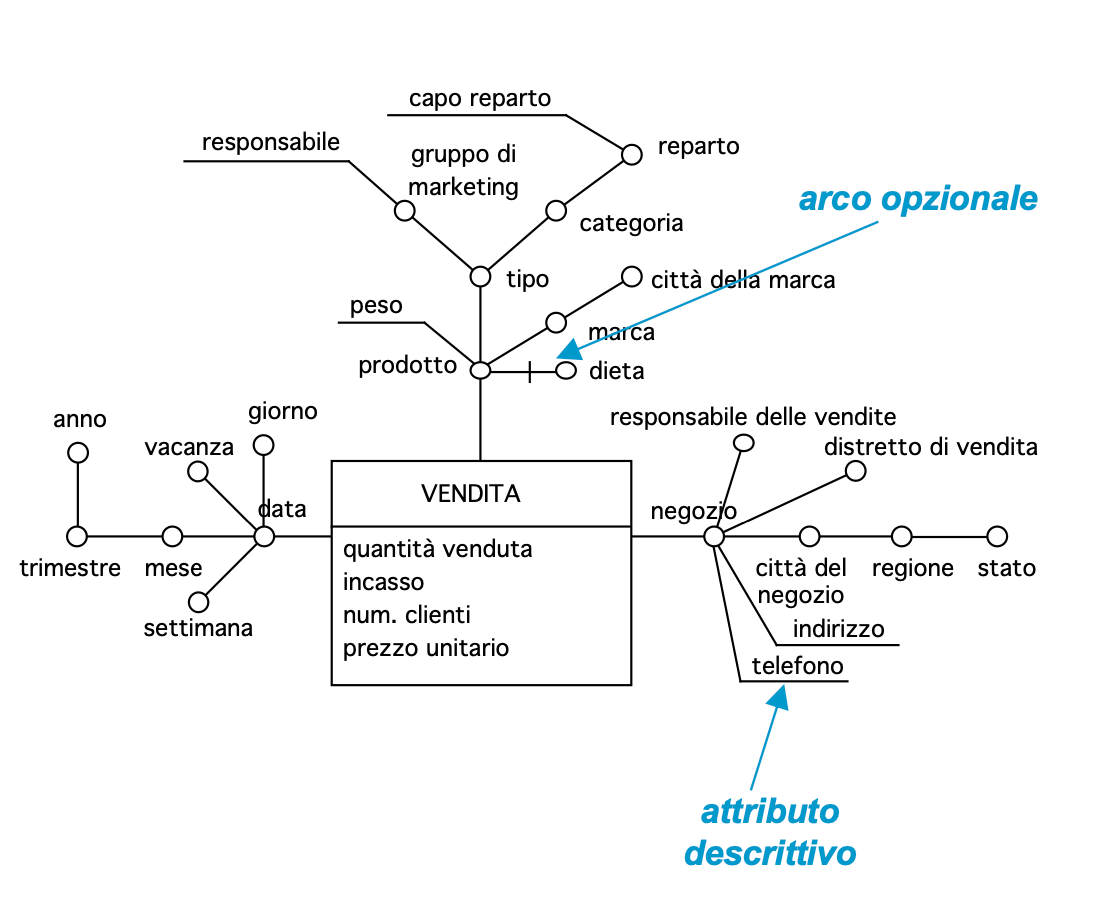
\includegraphics[width=0.6\linewidth]{img/descrittivo}
		\caption{Attributo descrittivo e arco opzionale}
		\label{fig:descr}
	\end{figure}
	\item 
	\textbf{Gerarchia condivisa}: in realtà le gerarchie possono avere dei cicli. Ho quattro modi per creare dei cicli nelle gerarchie del DFM, con quattro significati diversi. Il primo modo è la gerarchia condivisa, che è quello più debole, perché non pone vincoli sulle istanze. Una gerarchia condivisa è un albero che viene usato due o più volte all’interno dello stesso schema di fatto.
	\begin{figure}[H]
		\centering
		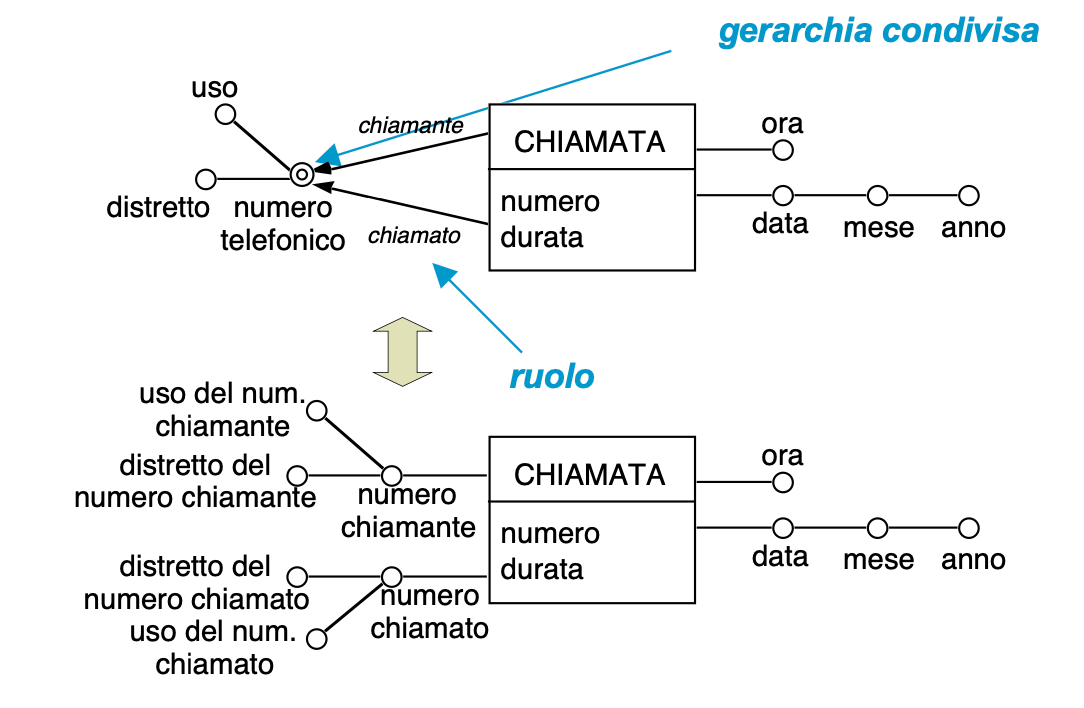
\includegraphics[width=0.6\linewidth]{img/condivisa}
		\caption{Gerarchia condivisa}
		\label{fig:condivisa}
	\end{figure}
	\item 
	\textbf{Convergenza}: aggiungo un vincolo sulle istanze. Mentre nel caso della condivisione non pongo vincoli sulle istanze, nel caso della convergenza non solo ho più percorsi che partono da un punto e arrivano nell’altro punto, ma qualunque dei due percorsi io prenda per ogni valore del punto di partenza arrivo sempre nello stesso punto di arrivo. Ho un vincolo aggiuntivo sulle istanze. 
	\begin{figure}[H]
		\centering
		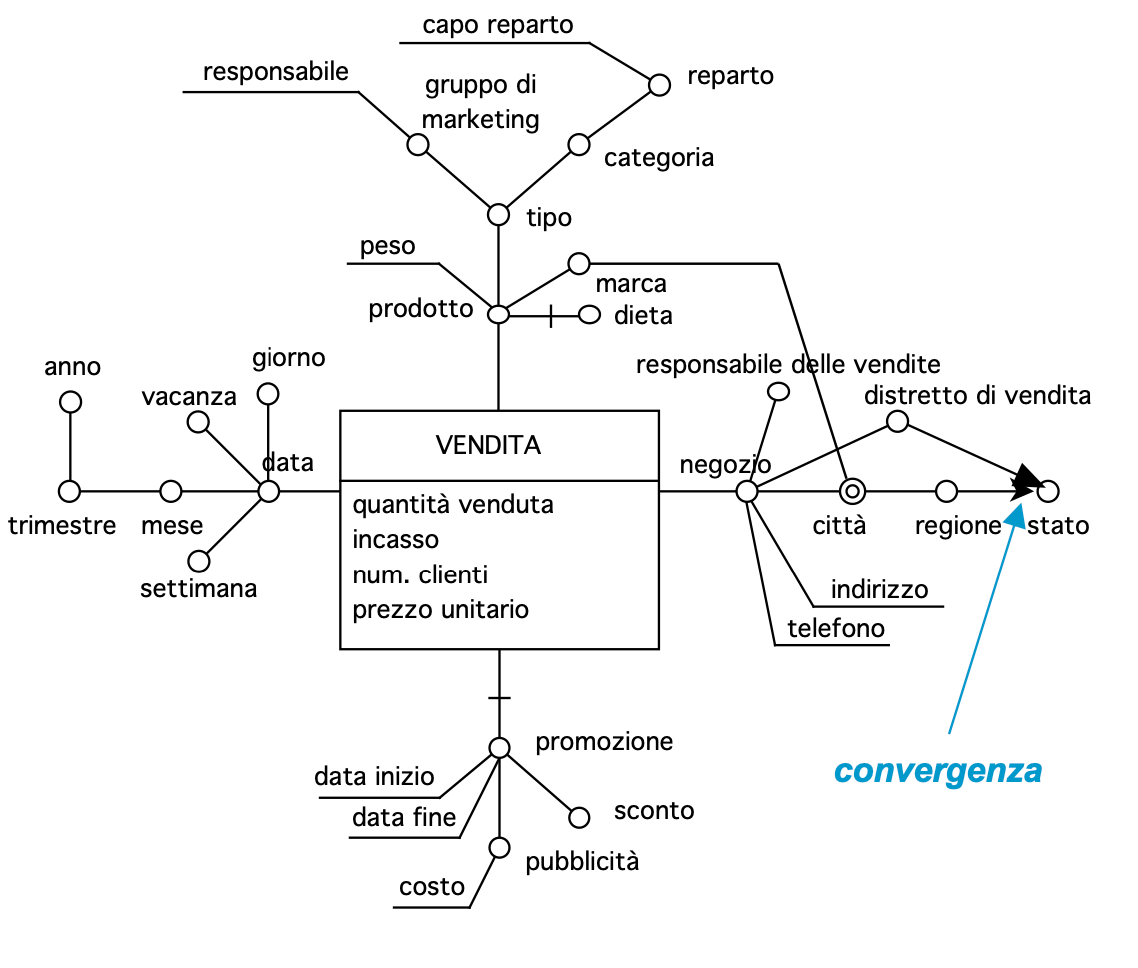
\includegraphics[width=0.6\linewidth]{img/convergenza}
		\caption{Convergenza}
		\label{fig:conv}
	\end{figure}
	\item 
	\textbf{Gerarchia incompleta}: per alcune istanze della gerarchia mancano dei valori di alcuni valori intermedi. La particolarità della gerarchia incompleta è che si hanno per le diverse istanze della gerarchia, un numero variabili di livelli pieni. 
		\begin{figure}[H]
		\centering
		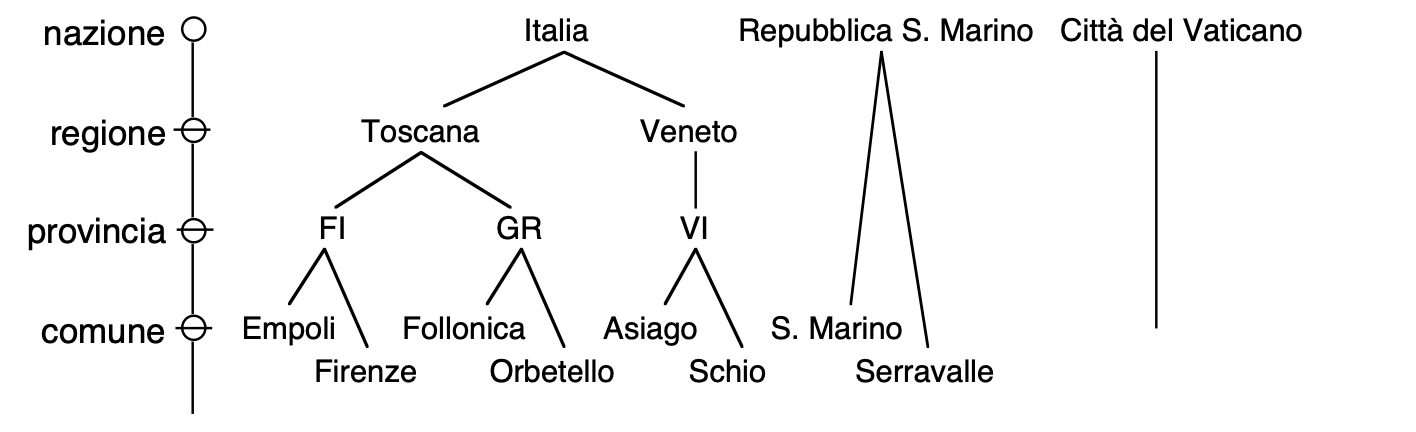
\includegraphics[width=0.7\linewidth]{img/incompleta}
		\caption{Gerarchia incompleta}
		\label{fig:incompleta}
	\end{figure}
	\item 
	\textbf{Additività}: esprime in che modo le misure possono essere aggregate. Di per sé le misure sono classificabili in tre categorie:
	\begin{itemize}
		\item 
		\textbf{Misure di flusso}: si riferiscono ad un periodo di tempo e vengono istanziate in modo cumulativo (il numero di prodotti venduti in un giorno, l’incasso mensile, il numero di nati in un anno). Sono quelle più semplice da gestire perché sono additive lungo tutte le dimensioni.
		\item 
		\textbf{Misure di livello}: vengono valutate in istanti di tempo (il numero di prodotti in inventario, il numero di abitanti di una città)
	\end{itemize}
	\item 
	\textbf{Misure unitarie}: vengono valutate in particolari istanti di tempo, ma sono espresse in termini relativi (il prezzo unitario di un prodotto, la percentuale di scoto, il cambio di una valuta) 
	
	La misura è detta \textbf{additiva} lungo una dimensione se i suoi valori possono essere aggregati lungo la corrispondente gerarchia tramite l’operatore di somma, altrimenti è detta non-additiva. Una misura \textbf{non-additiva} è non-aggregabile se nessun operatore di aggregazione può essere usato su di essa.  
	
	Uno schema di fatto si dice \textbf{vuoto} se non ha misure. In questo caso, il fatto registra solo il verificarsi di un evento.
	
	\subsection{Editing dell'albero}
	 
	
\end{itemize}
